\documentclass[runningheads,a4paper]{llncs}

\usepackage{fontspec}
\usepackage{polyglossia}
\setdefaultlanguage{russian}
\setotherlanguage{english}
\setmainfont{cmunrm.otf}[
  BoldFont = cmunbx.otf,
  ItalicFont = cmunti.otf,
  BoldItalicFont = cmunbi.otf
]
\setsansfont{cmunss.otf}[
  BoldFont = cmunsx.otf,
  ItalicFont = cmunsi.otf,
  BoldItalicFont = cmunso.otf
]
\setmonofont{cmuntt.otf}[
  BoldFont = cmuntb.otf,
  ItalicFont = cmunit.otf
]
\newfontfamily\cyrillicfont{cmunrm.otf}[
  BoldFont = cmunbx.otf,
  ItalicFont = cmunti.otf,
  BoldItalicFont = cmunbi.otf
]
\newfontfamily\cyrillicfontsf{cmunss.otf}[
  BoldFont = cmunsx.otf,
  ItalicFont = cmunsi.otf,
  BoldItalicFont = cmunso.otf
]
\newfontfamily\cyrillicfonttt{cmuntt.otf}[
  BoldFont = cmuntb.otf,
  ItalicFont = cmunit.otf
]

\usepackage{microtype}
\usepackage{graphicx}
\usepackage{booktabs}
\usepackage{tabularx}
\usepackage{array}
\usepackage{amsmath}
\usepackage{amssymb}
\usepackage{mathtools}
\usepackage{multirow}
\usepackage{placeins}
\usepackage{threeparttable}
\usepackage{siunitx}
\usepackage{xcolor}
\usepackage{hyperref}

\newcolumntype{L}{>{\raggedright\arraybackslash}X}
\newcolumntype{C}{>{\centering\arraybackslash}X}

\graphicspath{{figures/}}
\hypersetup{
  colorlinks=true,
  linkcolor=blue!50!black,
  urlcolor=blue!50!black,
  citecolor=blue!50!black,
  pdftitle={Углублённая доразметка и контролируемые пулы кандидатов в переоценке MS MARCO},
  pdfauthor={, , and }
}

\setlength{\emergencystretch}{1.5em}
\setlength{\tabcolsep}{5pt}
\renewcommand{\arraystretch}{1.12}
\sisetup{
  detect-all,
  input-decimal-markers = {.},
  table-number-alignment = center
}
\sloppy

\title{Углублённая доразметка и контролируемые пулы кандидатов в переоценке моделей ранжирования на коллекции MS MARCO}
\titlerunning{Углублённая доразметка и контролируемые пулы кандидатов}
\author{}
\authorrunning{}
\institute{}

\begin{document}

\maketitle
\begin{abstract}
В статье исследуется, как дополнительная ручная разметка влияет на оценку моделей информационного поиска на коллекции MS MARCO, где для большинства запросов исходно указан только один явно релевантный фрагмент текста. Для 1179 запросов и 33667 пар «запрос-документ» сравниваются исходная разметка, расширенная человеческая разметка и метки модели-судьи на базе MiniLM. Затем модель-судья применяется к полному набору запросов для анализа псевдоразметки в контролируемых пулах кандидатов. Показано, что на ручной подвыборке среднее число релевантных документов на запрос возрастает с 1.07 до 17.47, а NDCG@10 статистически значимо увеличивается для всех рассматриваемых источников ранжирования: например, с 0.597 до 0.877 для BM25 и с 0.701 до 0.967 для E5. Для полного набора установлено, что среднее число около 130 псевдорелевантных документов на запрос возникает при предъявлении модели-судье большого объединённого пула кандидатов из первых 200 результатов BM25, E5 и BGE; поэтому это число нельзя интерпретировать без описания способа формирования пула.

\keywords{информационный поиск \and MS MARCO \and mMARCO \and RusBEIR \and релевантностная разметка \and дополнительная разметка \and псевдоразметка \and пул кандидатов \and объединение ранжированных списков}
\end{abstract}

\section{Введение}

Для обучения современных нейросетевых моделей информационного поиска требуются большие наборы запросов, документов и оценок релевантности. Такие наборы данных позволяют обучать модели не только находить точные совпадения слов, но и учитывать семантическую близость запроса и документа. Одной из наиболее известных коллекций такого типа является MS MARCO, построенная на основе реальных поисковых запросов Bing и используемая для задач ранжирования фрагментов текста и документов \cite{bajaj2016msmarco}. На основе MS MARCO была создана многоязычная коллекция mMARCO, в которой исходные данные переведены на несколько языков, включая русский \cite{bonifacio2022mmarco}. Русская часть mMARCO используется в RusBEIR \textemdash{} русскоязычном бенчмарке для оценки моделей информационного поиска \cite{2025rusbeir}.

Важная особенность MS MARCO состоит в устройстве исходной разметки. В задаче ранжирования фрагментов текста для большинства запросов указан один положительный пример: фрагмент, который может содержать ответ на вопрос пользователя \cite{msmarco_datasets}. Это практично для создания большой коллекции, потому что полная ручная проверка миллионов фрагментов для сотен тысяч запросов была бы слишком дорогой. Однако такая разметка является неполной: если в корпусе существуют другие подходящие фрагменты, они могут отсутствовать в файлах эталонной разметки. Далее под эталонной разметкой понимаются таблицы вида «запрос-документ-метка релевантности», которые используются при вычислении метрик качества ранжирования.

Неполнота разметки особенно важна при сравнении моделей разных типов. Лексические методы, такие как BM25, опираются на совпадения слов \cite{robertson2009bm25}. Нейросетевые модели первичного поиска, такие как E5 и BGE, используют векторные представления запросов и документов \cite{wang2022e5,xiao2023cpack}. Модели типа cross-encoder оценивают пары «запрос-документ» совместно \cite{nogueira2019bert}. Эти подходы могут находить разные релевантные документы. Поэтому модель может вернуть полезный документ, но получить низкую оценку только потому, что этот документ отсутствует в исходной эталонной разметке. По этой причине переоценка MS MARCO после дополнительной разметки представляет самостоятельный исследовательский интерес.

В данной работе изучаются два уровня переоценки. Во-первых, анализируется ручная подвыборка, на которой доступна дополнительная человеческая разметка. Это позволяет сравнить исходную разметку MS MARCO с более плотной разметкой внутри одного и того же набора документов. Во-вторых, рассматривается полный набор запросов MS MARCO. Для него используется модель-судья: бинарный классификатор, который по паре «запрос-документ» выдаёт числовую оценку релевантности и затем, по заданному порогу, относит документ к релевантным или нерелевантным. Такая модель нужна потому, что вручную доразметить полный набор запросов практически невозможно.

Отдельно анализируется метод объединения рангов по обратным рангам (Reciprocal Rank Fusion, RRF) \cite{cormack2009rrf}. RRF объединяет несколько ранжированных списков: документ получает больший итоговый балл, если он находится высоко в выдаче нескольких систем. В работе RRF используется как дополнительная проверка того, повышает ли простое объединение выдач качество итогового ранжирования по сравнению с отдельными системами при одной и той же разметке.

Исследование структурировано вокруг трёх исследовательских вопросов.
\begin{enumerate}
\item \textbf{Вопрос 1.} Как дополнительная ручная разметка меняет плотность эталонной разметки и значения метрик качества поиска?
\item \textbf{Вопрос 2.} Насколько надёжна модель-судья как инструмент автоматической псевдоразметки?
\item \textbf{Вопрос 3.} Как глубина пулинга влияет на число псевдорелевантных документов и на качество выдачи после объединения ранжированных списков методом RRF?
\end{enumerate}

Под глубиной пулинга понимается число первых документов, которые берутся из выдачи каждой системы перед объединением. Например, при $K=10$ модель-судья получает объединение первых 10 документов каждой системы, а при $K=200$ \textemdash{} существенно более широкий объединённый пул. Поэтому плотность псевдоразметки в полном эксперименте является свойством протокола пулинга, а не только свойством корпуса или модели-судьи.

Основные результаты состоят в следующем. На ручной подвыборке дополнительная разметка статистически значимо повышает метрики качества поиска для всех рассматриваемых моделей. Модель-судья на базе MiniLM \cite{wang2020minilm,reimers2019sentencebert} показывает приемлемое качество бинарной классификации и позволяет построить псевдоразметку для полного набора запросов. На полном наборе MS MARCO показано, что высокая плотность псевдоразметки определяется не только свойствами корпуса, но и способом формирования пула кандидатов. Наконец, RRF даёт выигрыш только при небольшом пуле кандидатов; при расширении пула его преимущество исчезает.

\section{Связанные работы}

Коллекция MS MARCO была предложена как крупномасштабный набор данных, основанный на реальных поисковых запросах, и стала одним из стандартных тестовых стендов для ранжирования текстовых фрагментов \cite{bajaj2016msmarco}. Её многоязычная версия mMARCO была создана машинным переводом исходной коллекции и используется для обучения многоязычных моделей поиска \cite{bonifacio2022mmarco}. Для русского языка важен также бенчмарк RusBEIR, объединяющий переведенные, адаптированные и изначально русскоязычные наборы данных для оценки информационного поиска \cite{2025rusbeir}.

В качестве лексического базового метода в подобных постановках традиционно используется BM25 \textemdash{} вероятностная модель ранжирования, основанная на частотах терминов и нормализации длины документа \cite{robertson2009bm25}. Современные нейросетевые методы первичного поиска строятся на векторных представлениях текстов; к распространённым семействам плотных ретриверов относятся E5 \cite{wang2022e5} и BGE/FlagEmbedding \cite{xiao2023cpack}. Для переранжирования широко применяются модели типа cross-encoder, основанные на совместной обработке запроса и документа трансформерной моделью \cite{nogueira2019bert}.

При создании тестовых коллекций для информационного поиска широко используется пулинг: документы из верхних частей выдач нескольких систем объединяются и затем передаются экспертам для разметки \cite{voorhees2005trec}. Такой подход существенно сокращает стоимость разметки, но делает оценочную коллекцию зависимой от того, какие системы и какая глубина выдачи были включены в пул.

Отдельное направление связано с объединением нескольких ранжированных списков. Метод объединения рангов по обратным рангам был предложен как простой способ объединять выдачи разных поисковых систем без обучения дополнительных параметров \cite{cormack2009rrf}. В более поздних работах по гибридному поиску и поиску с генерацией ответов было показано, что RRF остаётся распространенным и практически полезным приемом, но его эффект зависит от состава объединяемых систем, глубины списков и параметров объединения \cite{bruch2023fusion,mackenzie2023anserini,rackauckas2024ragfusion}.

Наша работа не вводит новую поисковую модель. Её вклад состоит в переоценке уже известных моделей после дополнительной разметки, в анализе автоматической псевдоразметки с помощью модели-судьи и в явном разделении двух факторов: качества модели-судьи и размера объединённого пула кандидатов.

\section{Данные, пулинг и ручная доразметка}

\subsection{Исходная коллекция}

Исходным материалом является коллекция MS MARCO Passage Ranking. Она содержит запросы пользователей, корпус из 8841823 коротких текстовых фрагментов и файлы qrels, то есть файлы эталонной разметки, в которых для запроса указаны документы, считающиеся релевантными. В исходном файле qrels для development-части содержится 7437 положительных пар для 6980 запросов. Полный протокол пулинга, рассматриваемый в этой работе, крупнее: он использует 101093 запроса, для которых доступны сохранённые выдачи BM25, E5 и BGE для последующей псевдоразметки.

Проблема исходной разметки состоит не в том, что указанные положительные документы неверны, а в том, что они часто не исчерпывают все подходящие ответы в корпусе. Например, если запрос спрашивает, к какому округу относится некоторый населённый пункт или объект, в корпусе может быть несколько фрагментов, прямо называющих один и тот же округ. Исходная разметка может содержать только один из них. В таком случае поисковая система, которая вернула другой корректный фрагмент, получает заниженную оценку, потому что этот фрагмент отсутствует в эталонном файле.

\subsection{Формирование ручной подвыборки}

Чтобы исследовать проблему недоразметки, для выбранных запросов был выполнен пулинг кандидатов. В пул включались документы из верхних частей выдач нескольких источников: BM25 как лексического базового метода, E5 и BGE как плотных bi-encoder ретриверов, а также вспомогательного E5-сигнала, основанного на сходстве кандидата с уже известным релевантным ответом для данного запроса. Последний источник не является обычной поисковой системой, поскольку использует информацию, которой модель поиска не располагает в реальном сценарии: кроме текста запроса, ему известен исходный релевантный документ MS MARCO. Поэтому этот сигнал используется только для расширения пула разметки и не применяется в полном протоколе как самостоятельная модель поиска.

Для каждого запроса из выдачи каждого источника брались первые 10 документов, после чего эти списки объединялись в один пул кандидатов. Повторяющиеся документы удалялись, поэтому фактическое число документов на запрос обычно было меньше суммы четырёх списков. Затем документы из объединённого пула были дополнительно размечены человеком. При разметке эксперт видел не только запрос и оцениваемый документ, но и исходный релевантный ответ MS MARCO; благодаря этому новая разметка согласуется с исходной интерпретацией информационной потребности запроса.

Такая процедура позволяет сравнить три состояния одного и того же оценочного материала: исходную разметку MS MARCO, расширенную человеческую разметку и автоматическую разметку, которую позднее строит модель-судья.

\subsection{Характеристики нового датасета}

Полученная ручная подвыборка содержит 1179 запросов и 33667 пар «запрос-документ». В среднем на один запрос приходится 28.56 документа. В исходной разметке MS MARCO внутри этой подвыборки содержится 1257 положительных пар, то есть в среднем 1.07 релевантного документа на запрос. После дополнительной человеческой разметки число положительных пар возрастает до 20597, то есть до 17.47 релевантного документа на запрос. Таким образом, новый оценочный набор не заменяет MS MARCO, а показывает, насколько сильно меняется плотность разметки внутри специально сформированного пула кандидатов.

\begin{table}[t]
\centering
\caption{Состав ручного оценочного набора до и после дополнительной разметки.}
\label{tab:annotation-data}
\scriptsize
\setlength{\tabcolsep}{2pt}
\begin{tabularx}{\textwidth}{@{}>{\hsize=.86\hsize}L c c c c >{\hsize=1.14\hsize}L@{}}
\toprule
\textbf{Состояние} & \textbf{Запросы} & \textbf{Пары} & \textbf{Положит.} & \textbf{Рел./запрос} & \textbf{Комментарий} \\
\midrule
MS MARCO внутри пула & 1179 & 33667 & 1257 & 1.07 & исходные релевантные ответы \\
Ручная доразметка & 1179 & 33667 & 20597 & 17.47 & исходные и новые релевантные документы \\
Судья на том же пуле & 1179 & 33667 & 22193 & 18.82 & автоматическая разметка после обучения \\
\bottomrule
\end{tabularx}
\end{table}

В таблице~\ref{tab:annotation-data} видно, что основной эффект ручной доразметки состоит не в расширении числа запросов, а в резком росте плотности положительных оценок внутри уже сформированного пула кандидатов.

\begin{table}[t]
\centering
\caption{Pooled-NDCG@10 на ручной подвыборке до и после дополнительной человеческой разметки. Значения рассчитываются внутри размеченного пула кандидатов и не являются leaderboard-оценкой на полном корпусе.}
\label{tab:main}
\footnotesize
\setlength{\tabcolsep}{4pt}
\begin{tabularx}{\textwidth}{@{}L c c c L@{}}
\toprule
\textbf{Источник ранжирования} & \textbf{Исходная} & \textbf{После доразметки} & \textbf{$\Delta$} & \textbf{Примечание} \\
\midrule
BM25 & 0.597 & 0.877 & +0.280 & лексический поиск \\
E5 & 0.701 & 0.967 & +0.266 & нейросетевой поиск по запросу \\
BGE & 0.672 & 0.948 & +0.276 & нейросетевой поиск по запросу \\
E5 + исходный ответ & 0.708 & 0.975 & +0.267 & вспомогательный сигнал для пулинга \\
RRF & 0.607 & 0.906 & +0.299 & объединение ранжированных списков \\
\bottomrule
\end{tabularx}
\end{table}

Таблица~\ref{tab:main} показывает, что дополнительная разметка меняет не только плотность оценочного набора, но и измеряемое качество ранжирования. Вспомогательный сигнал «E5 + исходный ответ» ожидаемо даёт наибольшее значение на ручном пуле, поскольку использует исходный релевантный документ; поэтому его нельзя интерпретировать как самостоятельную поисковую модель для обычного сценария.

В дальнейшем эта ручная подвыборка используется для двух задач. Во-первых, на ней сравниваются значения метрик качества поиска при исходной и дополнительной разметке. Во-вторых, она служит обучающим и проверочным материалом для модели-судьи, которая затем применяется к более крупному набору запросов.

\section{Постановка задачи и экспериментальный протокол}

Пусть $\mathcal{Q}$ \textemdash{} множество запросов, $\mathcal{D}$ \textemdash{} корпус документов, а $\mathcal{M}$ \textemdash{} множество ранжирующих систем. Для запроса $q \in \mathcal{Q}$ и модели $m \in \mathcal{M}$ обозначим через $\mathrm{TopK}_m(q)$ множество первых $K$ документов в выдаче модели $m$. Тогда объединённый пул кандидатов определяется как
\begin{equation}
\label{eq:pool}
P_q^{(K)} = \bigcup_{m \in \mathcal{M}} \mathrm{TopK}_m(q).
\end{equation}

Параметр $K$ задаёт, сколько документов берётся из выдачи каждой отдельной системы: при $K=10$ используются первые 10 документов, при $K=200$ \textemdash{} первые 200 документов. После объединения и удаления повторов итоговый пул может содержать меньше чем $K \cdot |\mathcal{M}|$ документов.

На ручной подвыборке оцениваются четыре источника ранжирования внутри пула: BM25 как лексический базовый метод, E5 и BGE как плотные bi-encoder ретриверы и вспомогательный сигнал «E5 + исходный ответ». Первые три источника строят выдачу только по тексту запроса и поэтому могут применяться к полному набору запросов. Четвёртый источник использует исходный релевантный документ MS MARCO и нужен только для расширения ручного пула; в полном протоколе он не используется как самостоятельная поисковая система.

\subsection{Модель-судья}

Модель-судья нужна для переноса сигнала ручной разметки на пулы кандидатов, которые нельзя полностью проверить человеком. Она не заменяет BM25, E5 или BGE: эти системы формируют документы-кандидаты, а судья присваивает уже выбранным парам «запрос-документ» бинарные псевдометки релевантности. Поэтому судья оценивается как классификатор релевантности пар, а не как поисковая модель первого этапа на исходной эталонной разметке.

Модель-судья является cross-encoder моделью: запрос и документ-кандидат обрабатываются трансформером совместно. Этим она отличается от E5 и BGE, которые являются bi-encoder ретриверами и кодируют запросы и документы отдельно. В качестве судьи используется \texttt{cross-encoder/ms-marco-MiniLM-L-6-v2} \cite{wang2020minilm,reimers2019sentencebert}.\footnote{\url{https://huggingface.co/cross-encoder/ms-marco-MiniLM-L-6-v2}} Модель выбрана как компактная, публичная и уже обученная на MS MARCO. Базовая версия без дообучения достигает ROC-AUC 0.865 на нашей валидационной части; после дообучения на ручных метках ROC-AUC возрастает до 0.908. На вход судьи подаются только текст запроса и текст документа-кандидата; эмбеддинги, ранги и оценки BM25, E5, BGE или RRF не передаются.

Дообучение выполнялось на ручной подвыборке из 1179 запросов и 33667 пар. Разбиение на обучающую, валидационную и тестовую части проводилось по идентификаторам запросов в пропорции 70/15/15 с фиксированным случайным зерном 42: 23543 пары для 825 запросов вошли в обучение, 5122 пары для 177 запросов \textemdash{} в валидационную часть, 5002 пары для 177 запросов \textemdash{} в тестовую часть. Все документы одного запроса попадали только в одну часть. Это исключает утечку данных между обучением, подбором порога и итоговой проверкой. Порог бинаризации выбирался на валидационной части и в финальной конфигурации составил $\tau = -0.2187$.

Пусть $s_\theta(q,d)$ \textemdash{} численная оценка модели-судьи для пары «запрос-документ», а $\tau$ \textemdash{} порог бинаризации. Тогда решение модели-судьи задаётся выражением
\begin{equation}
\label{eq:judge}
\hat y_{\theta,\tau}(q,d) = \mathbb{I}\left[s_\theta(q,d) \ge \tau\right].
\end{equation}

Соответствующее множество псевдорелевантных документов внутри пула $P_q^{(K)}$ равно
\begin{equation}
\label{eq:positive-set}
R_q^{(K)} = \left\{ d \in P_q^{(K)} \; \middle| \; \hat y_{\theta,\tau}(q,d) = 1 \right\},
\end{equation}
а плотность положительных меток определяется как
\begin{equation}
\label{eq:density}
\rho_q^{(K)} = \frac{|R_q^{(K)}|}{|P_q^{(K)}|}.
\end{equation}

\subsection{Протокол для полного набора запросов}

Для полного набора запросов использовались сохранённые ранжированные списки BM25, E5 и BGE. Для каждой глубины пулинга $K \in \{10, 30, 50, 100, 200\}$ из первых $K$ результатов каждой системы строился объединённый пул \eqref{eq:pool}. Затем модель-судья оценивала все пары «запрос-документ» из этого пула и по порогу $\tau$ формировала псевдоразметку. Поэтому результаты полного протокола зависят не только от модели-судьи, но и от того, сколько кандидатов было предъявлено ей на оценку.

\begin{figure}[t]
\centering
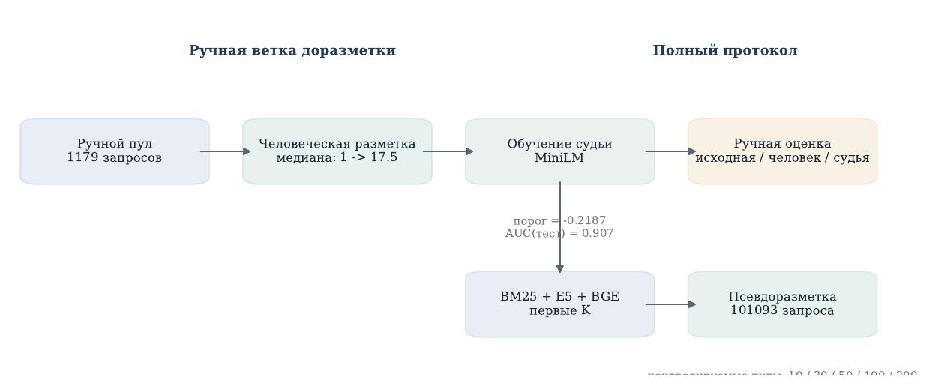
\includegraphics[width=0.92\textwidth,trim=0 18pt 0 0,clip]{protocol_schematic.pdf}
\caption{Схема экспериментального протокола. Верхняя ветка соответствует ручной доразметке и обучению модели-судьи, нижняя ветка \textemdash{} протоколу для полного набора запросов с контролируемыми пулами кандидатов. Рисунок подчёркивает, что выводы по ручной подвыборке и по полному набору относятся к различным, хотя и связанным, постановкам.}
\label{fig:protocol}
\end{figure}

Рисунок~\ref{fig:protocol} подчёркивает принципиальное различие между ручной и полной постановками. На ручной подвыборке плотность эталонной разметки повышается внутри относительно небольшого пула документов. На полном наборе модель-судья получает существенно больший пул, поэтому высокая плотность псевдоразметки не может интерпретироваться вне контекста выбранного $K$.

\section{Метрики и проверка значимости}

Основной целевой метрикой в работе выступает NDCG@10, то есть нормализованная дисконтированная накопленная полезность на первых десяти позициях выдачи. Для запроса $q$ она рассчитывается через
\begin{align}
\label{eq:dcg}
\mathrm{DCG}@10(q) &= \sum_{i=1}^{10} \frac{2^{\mathrm{rel}_i(q)} - 1}{\log_2(i + 1)}, \\
\label{eq:ndcg}
\mathrm{NDCG}@10(q) &= \frac{\mathrm{DCG}@10(q)}{\mathrm{IDCG}@10(q)}.
\end{align}

Для объединения ранжированных списков используется классический метод RRF:
\begin{equation}
\label{eq:rrf}
\mathrm{RRF}(d \mid q) = \sum_{m \in \mathcal{M}} \frac{1}{c + \mathrm{rank}_m(d,q)}, \qquad c = 60.
\end{equation}

Попарные сравнения выполняются на уровне запросов с помощью парного перестановочного теста. Для двух систем $A$ и $B$ вводится разность
\begin{equation}
\label{eq:delta}
\Delta_q = \mathrm{NDCG}_A(q) - \mathrm{NDCG}_B(q),
\end{equation}
а наблюдаемая статистика имеет вид
\begin{equation}
\label{eq:perm}
T = \frac{1}{|\mathcal{Q}'|} \sum_{q \in \mathcal{Q}'} \Delta_q,
\end{equation}
где $\mathcal{Q}'$ \textemdash{} множество запросов, для которых обе системы имеют корректную оценку. При перестановочном тесте знаки $\Delta_q$ случайно инвертируются, а $p$-значение оценивается как доля перестановок, для которых модуль полученной статистики не меньше наблюдаемого.

Такая постановка важна по двум причинам. Во-первых, она проверяет различия между системами на уровне запросов, а не только по средним. Во-вторых, она позволяет корректно интерпретировать небольшие, но устойчивые отличия, например выигрыш RRF над E5 на узком пуле полного протокола.

\section{Результаты углублённой доразметки}

\subsection{Сдвиг плотности эталонной разметки}

Первый центральный результат состоит в том, что углублённая доразметка радикально меняет плотность эталонной разметки. На ручной части среднее число релевантных документов на запрос возрастает с 1.07 до 17.47, а медиана \textemdash{} с 1 до 17.5. Для автоматической разметки, полученной моделью-судьей на ручной подвыборке, медиана дополнительно возрастает до 19. На псевдоразметке полного набора медиана достигает 93, а 99-й процентиль \textemdash{} 401.

Число порядка 130 псевдорелевантных документов на запрос не следует интерпретировать как прямую оценку «истинной» релевантности корпуса. Это число возникает в полном протоколе при $K=200$, где средний размер пула составляет 451.54 документа на запрос. Следовательно, наблюдаемая плотность связана как с качеством модели-судьи, так и с протоколом предъявления кандидатов.

\subsection{Изменение качества ранжирования}

На ручной подвыборке углублённая доразметка статистически значимо повышает NDCG@10 для всех источников ранжирования внутри пула. Это относится как к лексическому базовому методу, так и к нейросетевому первичному поиску, вспомогательному сигналу с исходным ответом и RRF. Автоматическая разметка, полученная моделью-судьей на ручной части, дополнительно увеличивает значения метрики, однако для интерпретации этих результатов важно отличать её от человеческих меток, поскольку она уже включает ошибку автоматической модели.

\begin{figure}[t]
\centering
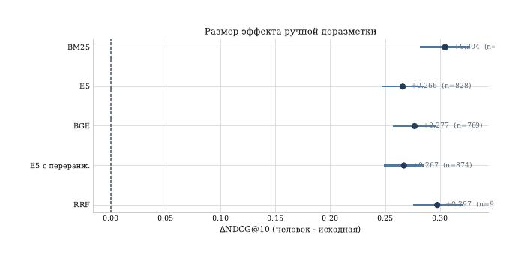
\includegraphics[width=\columnwidth]{manual_effect_forest.pdf}
\caption{Оценки размера эффекта для перехода от исходной разметки к дополнительной человеческой разметке. Точки показывают средний прирост NDCG@10 на уровне запросов, отрезки соответствуют 95\% доверительным интервалам, полученным бутстрэпом.}
\label{fig:effect-forest}
\end{figure}

\begin{table}[t]
\centering
\caption{Парные оценки размера эффекта на уровне запросов для перехода от исходной разметки к дополнительной человеческой разметке.}
\label{tab:effect-ci}
\footnotesize
\begin{tabularx}{\columnwidth}{Lccc}
\toprule
\textbf{Модель} & \textbf{$\Delta$NDCG@10} & \textbf{95\% ДИ} & \textbf{Число запросов} \\
\midrule
BM25 & +0.304 & [0.281; 0.328] & 499 \\
E5 & +0.266 & [0.247; 0.286] & 828 \\
BGE & +0.277 & [0.257; 0.296] & 769 \\
E5 + исходный ответ & +0.267 & [0.249; 0.285] & 874 \\
RRF & +0.297 & [0.275; 0.320] & 952 \\
\bottomrule
\end{tabularx}
\end{table}

\noindent Значения в таблице~\ref{tab:effect-ci} рассчитаны как средние парные различия на тех запросах, где для соответствующей модели определены обе оценки. Поэтому они могут немного отличаться от простой разности средних значений в таблице~\ref{tab:main}, где для каждого столбца используется весь доступный набор запросов.

Из таблиц~\ref{tab:main} и \ref{tab:effect-ci}, а также рисунка~\ref{fig:effect-forest} следует, что рост при переходе от исходной к дополнительной человеческой разметке носит систематический характер. В парном расчёте на общих запросах для BM25 прирост составляет $+0.304$, для E5 \textemdash{} $+0.266$, для BGE \textemdash{} $+0.277$, для вспомогательного сигнала «E5 + исходный ответ» \textemdash{} $+0.267$, для RRF \textemdash{} $+0.297$. Во всех перечисленных случаях парный перестановочный тест даёт $p < 0.001$, а 95\% доверительные интервалы прироста на уровне запросов не пересекают нулевую линию.

Важно также, что на ручной подвыборке RRF не становится лучшей конфигурацией. На дополнительной человеческой разметке вспомогательный сигнал «E5 + исходный ответ» достигает 0.975, тогда как RRF даёт 0.906. Это ожидаемо, поскольку вспомогательный сигнал использует исходный релевантный ответ и поэтому имеет преимущество, недоступное обычным поисковым системам.

\subsection{Качество модели-судьи}

Модель-судья на базе MiniLM выступает не как финальная сильнейшая архитектура, а как воспроизводимый базовый инструмент для автоматической оценки релевантности. Несмотря на сравнительно лёгкую основу модели, качество судьи оказывается достаточным для анализа полного набора запросов.

\begin{figure}[t]
\centering
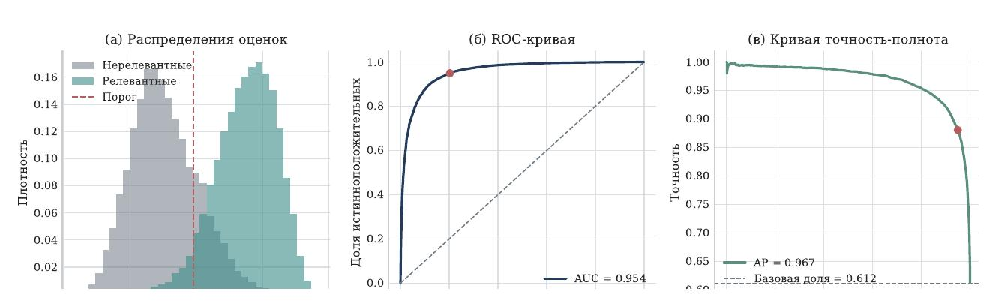
\includegraphics[width=0.95\textwidth]{judge_score_diagnostics.pdf}
\caption{Диагностика численных оценок модели-судьи на аннотированной ручной части. Показаны распределения оценок для релевантных и нерелевантных пар, ROC-кривая и кривая точность-полнота; красной точкой отмечено положение выбранного порога. Эта визуальная диагностика дополняет независимые метрики на отложенной выборке, но не заменяет их.}
\label{fig:judge}
\end{figure}

Согласно независимой оценке на отложенной выборке, модель-судья достигает площади под ROC-кривой (AUC) 0.908 на валидационной части и 0.907 на тестовой части, F1 0.875 на тестовой части и коэффициента согласия Коэна $\kappa = 0.636$ на отложенной выборке. Дополнительно модель покрывает 95.05\% ручных релевантных пар и даёт точность 87.97\% относительно человеческих меток. Рисунок~\ref{fig:judge} показывает, что даже на уровне численных оценок наблюдается хорошее разделение положительных и отрицательных пар; это делает MiniLM-судью достаточным базовым инструментом для первой статьи, хотя не исключает последующего сравнения с более мощными моделями переранжирования.

Выбранный рабочий порог также важен для интерпретации результатов. На аннотированной ручной части порог $\tau = -0.2187$ соответствует точности $0.881$, полноте $0.949$, F1 $0.914$ и доле предсказанных релевантных пар $0.660$. Эти значения не следует смешивать с метриками обобщающей способности на отложенной выборке: они характеризуют положение рабочего порога на размеченном пуле кандидатов.

\section{Псевдоразметка полного набора и контролируемые пулы}

Постановка для полного набора показывает, что свойства псевдоразметки необходимо анализировать совместно с глубиной объединённого пула кандидатов. Для $K=10$ среднее число кандидатов на запрос равно 21.88, а среднее число документов, отнесённых моделью-судьей к релевантным, \textemdash{} 14.19. Для $K=200$ эти значения увеличиваются до 451.54 и 128.64 соответственно, тогда как доля положительных меток снижается с 0.649 до 0.285.

\begin{figure}[t]
\centering
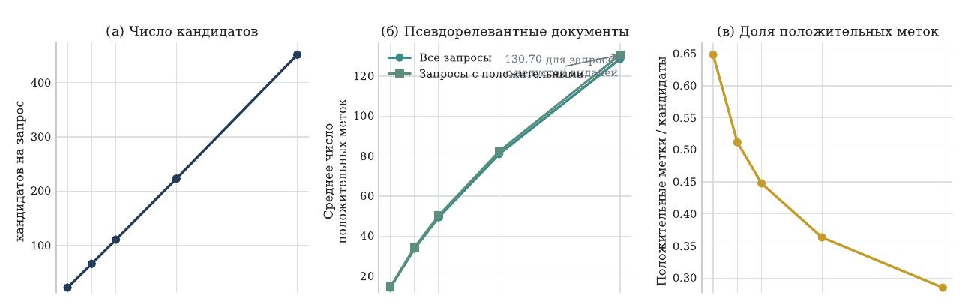
\includegraphics[width=0.94\textwidth]{pool_scaling_multipanel.pdf}
\caption{Изменение свойств псевдоразметки полного набора при увеличении размера объединённого пула кандидатов. Рисунок показывает, что рост числа псевдорелевантных документов следует рассматривать одновременно с ростом числа предъявленных кандидатов и с падением доли положительных меток.}
\label{fig:pool-scaling}
\end{figure}

\begin{figure}[t]
\centering
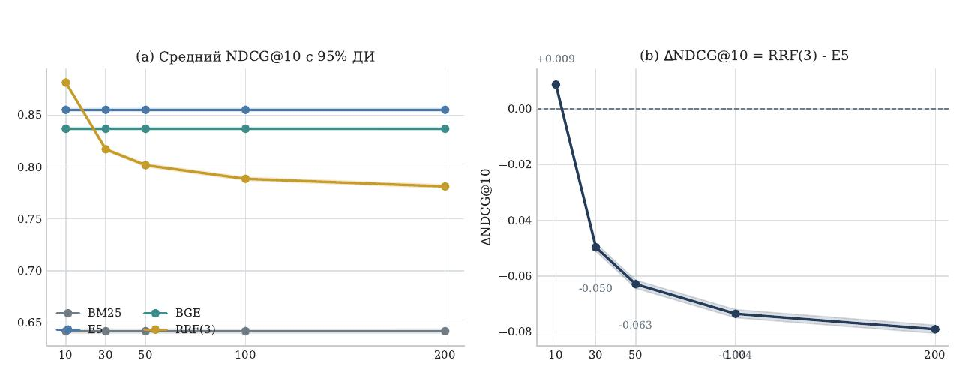
\includegraphics[width=0.94\textwidth]{fullset_uncertainty_panels.pdf}
\caption{Оценка неопределённости в полном протоколе. Слева показаны средние значения NDCG@10 с 95\% доверительными интервалами, полученными бутстрэпом, для BM25, E5, BGE и RRF(3) при различных глубинах пулинга. Справа приведена разность $\Delta$NDCG@10 между RRF(3) и E5, демонстрирующая смену знака при переходе от пула первых 10 результатов к более крупным пулам.}
\label{fig:fullset-uncertainty}
\end{figure}

Рисунки~\ref{fig:pool-scaling} и \ref{fig:fullset-uncertainty} отражают главный вывод полной части. На узком пуле при $K=10$ RRF даёт лучший результат среди доступных конфигураций полного протокола: 0.881 против 0.855 у E5 и 0.837 у BGE. Однако при увеличении $K$ качество RRF монотонно снижается: 0.817 для $K=30$, 0.802 для $K=50$, 0.789 для $K=100$ и 0.781 для $K=200$. Правая панель рисунка~\ref{fig:fullset-uncertainty} показывает, что разность «RRF минус E5» имеет положительный знак только при $K=10$ ($\Delta = +0.0087$, 95\% доверительный интервал $[0.0075; 0.0098]$), тогда как уже при $K=30$ становится отрицательной и далее лишь увеличивается по модулю. Следовательно, рост плотности эталонной разметки не эквивалентен росту качества ранжирования, а тезис о силе метода объединения оказывается чувствителен к протоколу отбора кандидатов.

\begin{table}[t]
\centering
\caption{Ключевые попарные сравнения, подтверждающие основные выводы статьи.}
\label{tab:sig}
\scriptsize
\setlength{\tabcolsep}{3pt}
\begin{tabularx}{\columnwidth}{@{}L c c c@{}}
\toprule
\textbf{Сравнение} & \textbf{$\Delta$ NDCG@10} & \textbf{$p$-значение} & \textbf{Число запросов} \\
\midrule
RRF на человеческой разметке против BM25 & +0.0372 & $< 0.001$ & 1102 \\
RRF на человеческой разметке против E5 & -0.0582 & $< 0.001$ & 1171 \\
RRF на человеческой разметке против E5 + исходный ответ & -0.0680 & $< 0.001$ & 1175 \\
RRF при $K=10$ против E5 & +0.0087 & $< 0.001$ & 95517 \\
RRF при $K=200$ против E5 & -0.0791 & $< 0.001$ & 98527 \\
\bottomrule
\end{tabularx}
\end{table}

Таблица~\ref{tab:sig} подтверждает два связанных вывода. Во-первых, на дополнительной человеческой разметке RRF статистически уступает вспомогательному сигналу, использующему исходный релевантный ответ. Во-вторых, на псевдоразметке полного набора знак преимущества RRF над E5 меняется при переходе от $K=10$ к $K=200$. Следовательно, тезис о «силе» метода объединения зависит от протокола отбора кандидатов и не может переноситься между постановками без дополнительных оговорок.

\section{Угрозы валидности и обсуждение}

Полученные результаты требуют аккуратной интерпретации с точки зрения валидности экспериментальной постановки.

\paragraph{Конструктивная валидность.} Углублённая доразметка меняет не только абсолютные значения метрик, но и саму сравнительную картину между моделями. Это означает, что разреженная эталонная разметка в MS MARCO может существенно занижать качество сильных моделей первичного поиска и переранжирования. Вместе с тем и человеческая разметка, и псевдоразметка зависят от того, какие документы были предъявлены на оценку.

\paragraph{Валидность протокола.} Псевдоразметку высокой плотности на полном наборе нельзя обсуждать в отрыве от размера объединённого пула кандидатов. Число порядка 130 положительных оценок на запрос является свойством конкретного полного протокола, а не «естественной» характеристикой корпуса MS MARCO. Именно поэтому в статье используется анализ контролируемых пулов, а не единичное число без оговорок.

\paragraph{Валидность модели-судьи.} Анализ модели-судьи в основной части использует два типа свидетельств: метрики классификации на отложенной выборке и диагностику численных оценок на аннотированной ручной части. Эти свидетельства взаимодополняют друг друга, но не эквивалентны: ROC-кривая, кривая точность-полнота и анализ чувствительности к порогу характеризуют рабочее поведение судьи на доступной разметке, тогда как AUC и F1 на отложенной выборке отражают его обобщающую способность.

Выбранный MiniLM cross-encoder является воспроизводимой базовой моделью, а не заведомо сильнейшим судьёй. Более крупные модели переранжирования, включая cross-encoder варианты BGE, а также судья, получающий известный релевантный ответ и документ-кандидат, требуют отдельного сравнения. В полном протоколе такой сигнал намеренно не используется: известный релевантный документ дал бы судье внешнюю подсказку, недоступную обычной поисковой модели, работающей только по запросу.

\paragraph{Внешняя валидность.} Полная часть статьи ограничена конфигурацией из трёх систем, которые строят выдачу только по запросу: BM25, E5 и BGE. Вспомогательный сигнал с исходным релевантным ответом используется только при ручном пулинге и не переносится на полный корпус как обычная модель поиска. Кроме того, все выводы относятся к коллекции MS MARCO и к конкретному протоколу отбора кандидатов; перенос их на другие корпуса требует отдельной проверки.

\paragraph{Практическое обсуждение.} Несмотря на эти ограничения, результаты дают устойчивый вывод по всем трём исследовательским вопросам. Для \textbf{вопроса 1} показано, что углублённая доразметка статистически повышает NDCG@10 и меняет плотность эталонной разметки. Для \textbf{вопроса 2} показано, что модель-судья на базе MiniLM имеет достаточное качество для базовой автоматической псевдоразметки, но требует контроля порога и проверки на отложенной выборке. Для \textbf{вопроса 3} установлено, что интерпретация числа 130.7 неотделима от глубины пулинга, а RRF полезен только в пределах небольшого контролируемого пула и не является универсально сильным методом объединения.

\section{Заключение}

В статье показано, что углублённая доразметка на MS MARCO приводит к существенному изменению плотности эталонной разметки и к статистически значимому росту NDCG@10 для всех рассмотренных источников ранжирования. На ручной подвыборке наибольшее значение достигает вспомогательный сигнал с исходным релевантным ответом, тогда как среди обычных поисковых систем лучшим остаётся E5. Модель-судья на базе MiniLM обеспечивает достаточно точный базовый инструмент для автоматической генерации псевдоразметки.

В полном эксперименте для автоматической псевдоразметки сознательно используется жёсткое ограничение: судья получает запрос и документ-кандидат, но не исходный релевантный ответ MS MARCO. Это сохраняет сопоставимость протокола с обычными поисковыми выдачами и не даёт судье внешнюю подсказку, недоступную поисковой модели во время ранжирования. В то же время результаты ручного пулинга показывают, что известный релевантный ответ является сильным сигналом. Поэтому естественное направление дальнейшей работы состоит в изучении модели-судьи с форматом входа «запрос, известный верный ответ, документ или ответ для оценки» и в сравнении такой модели с более сильными cross-encoder архитектурами.

Для полного протокола установлено, что глубина пулинга является ключевым фактором интерпретации результатов. При небольшом объединённом пуле RRF даёт лучший результат среди доступных конфигураций, однако при расширении пула кандидатов его качество монотонно снижается. Следовательно, показатели плотности псевдоразметки и выигрыша методов объединения должны анализироваться не изолированно, а вместе с протоколом отбора кандидатов.

Практический вывод состоит в том, что псевдоразметка на полном корпусе полезна как исследовательский инструмент, но требует анализа контролируемых пулов и явных ограничений в формулировке выводов. В этом смысле переоценка MS MARCO должна обсуждаться не только как улучшение разметки, но и как уточнение самого протокола измерения качества.

\begin{thebibliography}{99}

\bibitem{bajaj2016msmarco}
P.~Bajaj, D.~Campos, N.~Craswell, L.~Deng, J.~Gao, X.~Liu, R.~Majumder, A.~McNamara, B.~Mitra, T.~Nguyen, M.~Rosenberg, X.~Song, A.~Stoica, S.~Tiwary, T.~Wang.
\newblock \textit{MS MARCO: A Human Generated MAchine Reading COmprehension Dataset}.
\newblock arXiv preprint arXiv:1611.09268, 2016.

\bibitem{msmarco_datasets}
Microsoft.
\newblock \textit{MS MARCO datasets}.
\newblock \url{https://microsoft.github.io/msmarco/}, accessed 2026.

\bibitem{bonifacio2022mmarco}
L.~Bonifacio, V.~Jeronymo, H.~Queiroz Abonizio, I.~Campiotti, M.~Fadaee, R.~Lotufo, R.~Nogueira.
\newblock \textit{mMARCO: A Multilingual Version of MS MARCO Passage Ranking Dataset}.
\newblock arXiv preprint arXiv:2108.13897, 2021.

\bibitem{2025rusbeir}
G.~, M.~Tikhomirov, E.~Kozhevnikov, M.~Kornilov, N.~.
\newblock \textit{Building Russian Benchmark for Evaluation of Information Retrieval Models}.
\newblock Computational Linguistics and Intellectual Technologies, 2025.

\bibitem{robertson2009bm25}
S.~E. Robertson, H.~Zaragoza.
\newblock \textit{The Probabilistic Relevance Framework: BM25 and Beyond}.
\newblock Foundations and Trends in Information Retrieval, 3(4):333\textendash{}389, 2009.

\bibitem{wang2022e5}
L.~Wang, N.~Yang, X.~Huang, B.~Jiao, L.~Yang, D.~Jiang, R.~Majumder, F.~Wei.
\newblock \textit{Text Embeddings by Weakly-Supervised Contrastive Pre-training}.
\newblock arXiv preprint arXiv:2212.03533, 2022.

\bibitem{xiao2023cpack}
S.~Xiao, Z.~Liu, P.~Zhang, N.~Muennighoff, D.~Lian, J.-Y. Nie.
\newblock \textit{C-Pack: Packed Resources for General Chinese Embeddings}.
\newblock arXiv preprint arXiv:2309.07597, 2023.

\bibitem{nogueira2019bert}
R.~Nogueira, K.~Cho.
\newblock \textit{Passage Re-ranking with BERT}.
\newblock arXiv preprint arXiv:1901.04085, 2019.

\bibitem{wang2020minilm}
W.~Wang, F.~Wei, L.~Dong, H.~Bao, N.~Yang, M.~Zhou.
\newblock \textit{MiniLM: Deep Self-Attention Distillation for Task-Agnostic Compression of Pre-Trained Transformers}.
\newblock Advances in Neural Information Processing Systems, 33:5776\textendash{}5788, 2020.

\bibitem{reimers2019sentencebert}
N.~Reimers, I.~Gurevych.
\newblock \textit{Sentence-BERT: Sentence Embeddings using Siamese BERT-Networks}.
\newblock In \textit{Proceedings of EMNLP-IJCNLP}, pp.~3982\textendash{}3992, 2019.

\bibitem{cormack2009rrf}
G.~V. Cormack, C.~L.~A. Clarke, S.~B{\"u}ttcher.
\newblock \textit{Reciprocal Rank Fusion outperforms Condorcet and Individual Rank Learning Methods}.
\newblock In \textit{Proceedings of the 32nd Annual International ACM SIGIR Conference on Research and Development in Information Retrieval}, pp.~758\textendash{}759, 2009.

\bibitem{voorhees2005trec}
E.~M. Voorhees, D.~K. Harman.
\newblock \textit{TREC: Experiment and Evaluation in Information Retrieval}.
\newblock MIT Press, 2005.

\bibitem{bruch2023fusion}
S.~Bruch, S.~Gai, A.~Ingber.
\newblock \textit{An Analysis of Fusion Functions for Hybrid Retrieval}.
\newblock arXiv preprint arXiv:2210.11934, 2022.

\bibitem{mackenzie2023anserini}
X.~Ma, T.~Teofili, J.~Lin.
\newblock \textit{Anserini Gets Dense Retrieval: Integration of Lucene's HNSW Indexes}.
\newblock In \textit{Proceedings of the 32nd ACM International Conference on Information and Knowledge Management}, 2023.

\bibitem{rackauckas2024ragfusion}
Z.~Rackauckas.
\newblock \textit{RAG-Fusion: A New Take on Retrieval-Augmented Generation}.
\newblock International Journal on Natural Language Computing, 13(1), 2024.

\end{thebibliography}

\end{document}
